\documentclass[11pt,a4paper]{article}
\usepackage[utf8]{inputenc}
\usepackage[T1]{fontenc}
\usepackage{amsfonts}
\usepackage[french]{babel}
\frenchbsetup{StandardLists=true} % à inclure si on utilise \usepackage[francais]{babel}
\usepackage{enumitem}
\usepackage{amssymb}
\usepackage{amsmath}
\usepackage[left=2cm,right=2cm,top=2cm,bottom=2cm]{geometry}
\usepackage{multirow}
\usepackage[dvipsnames]{xcolor}
\usepackage{gensymb} %symbole degré

\usepackage[T1]{fontenc}
\usepackage{fouriernc}
\usepackage{graphicx}

\usepackage{setspace}
\singlespacing

\usepackage{pstricks}
\usepackage{xkeyval}
\usepackage{pst-labo}
\usepackage{chemist} %chimie

\usepackage{tcolorbox}
\usepackage{multicol}
\usepackage{caption}
\usepackage{fancyhdr}
\pagestyle{fancy}
\renewcommand\headrulewidth{1pt}
\fancyhead[L]{Lycée Denis Diderot }
\fancyhead[R]{Classe de 1 Bac Pro }
\setcounter{page}{1}\fancyfoot[C]{page \thepage}
\fancyfoot[R]{Année 2024-2025}
\fancyfoot[L]{Alexis RUIZ}
\usepackage{multirow,tabularx,booktabs}
\usepackage[tikz]{bclogo} 

\newcommand{\cadreblanc}[1]{%
\medskip\framebox[\linewidth][c]{%
\rule{0mm}{#1mm}}\par
\medskip}

\usepackage{awesomebox}
\setlength{\aweboxvskip}{0mm}
\usepackage{pifont}
\usepackage{chemmacros}
\chemsetup{modules=all}
\setlength{\columnseprule}{.25mm}

\renewcommand{\arraystretch}{2.5}
\newcommand*\acocher{\quitvmode{\fboxsep0pt \fboxrule0.8pt \fbox{\vrule height1.8ex depth.1ex width0pt \vrule height0pt depth0pt width1.9ex }}}

\newcolumntype{C}[1]{>{\centering\arraybackslash }b{#1}}

\newcommand{\code}{\awesomebox[black]{2pt}{

\includegraphics[scale=0.15]{../Chapitre 1 - Energie et puissance électrique/images/frame.png}
}{black}}

\newcommand{\moteur}{\awesomebox[black]{2pt}{

\includegraphics[scale=1]{images/moteur.jpg} 
}{black}}

\newcommand{\defconclusion}{\awesomebox[black]{2pt}{\rotatebox{90}{\Large{\textbf{Conclusion}}}}{black}}

\newcommand{\defbox}{\awesomebox[black]{2pt}{
\includegraphics[scale=0.5]{../Chapitre 1 - Energie et puissance électrique/images/appel exam.png}}{black}}

  \newenvironment{itemize*}%  % listes compactes
    {\begin{termite}%
      \setlength{\itemsep}{0pt}%
      \setlength{\parskip}{0pt}}%
    {\end{itemize}}

\frenchbsetup{StandardLists=true}
%%%%%%%%%%%%%%%%%%%%%%%%%%%%%%%%%%%

\begin{document}
%%%%%%%%%%%%%%%%%%%%%%%%%

\flushleft \textbf{NOM : \hfill Classe : \hspace{3cm} ~~\\[2mm]
Prénom:\\[0,4cm]
}
\hrule\
\\[0,2cm]

\begin{center}
 \LARGE{TP4 - Dosage pH-métrique du vinaigre    }
\end{center}

\vspace{3 mm}

\normalsize

\hrule\
\\[0,2cm]
   \begin{center}
   \textbf{Le soin et la rédaction interviendront dans la notation.}
   \end{center} 
%%%%%%%%%%%%%%%%%%%%%%%%%%%
\noindent%
\begin{minipage}{.45\textwidth}%
Le vinaigre contient un acide (qui se nomme acide éthanoïque de formule chimique \chemform{CH_3COOH}). Les bouteilles du commerce sont vendues avec une unité de mesure de cet acide que l'on nomme le degré d'acidité. Les vinaigres de type "cristal" (incolore) sont vendus avec un titre $d=8\%$ en acide. Ce qui correspond à 8 g d'acide éthanoïque pour 100 g de vinaigre. L'objectif du TP est de vérifier ce degré. \\

\vspace{0.5cm}

Nous allons doser cet acide par de la soude NaOH de concentration \chemform{C_B=0,1 mol/L} 


\end{minipage}%
\hfill
\begin{minipage}{.5\textwidth}%
    
 \begin{bclogo}[couleur=white,  arrondi =0.1 , logo = \bcinfo, epBarre =2]{ Matériel }

\begin{itemize*}

\item Pipette jaugée \SI{10}{\milli\liter} avec son dispositif d'aspiration.  

\item 1 bécher de \SI{100}{\milli\liter}.

\item 1 bécher de \SI{100}{\milli\liter} étiqueté soude.

\item 1 bécher de \SI{100}{\milli\liter} Solution A.

\item 1 bécher de \SI{100}{\milli\liter} étiqueté vinaigre. 

\item 1 bécher de \SI{250}{\milli\liter}, récupération des produits usagés. 

\item 1 erlen-meyer de \SI{250}{\milli\liter}, étiqueté dosage. 


\item 1 Fiole jaugée de 100 mL

\item  Une burette graduée \SI{25}{\milli\liter} avec son support 

\item Agitateur magnétique avec un barreau aimanté

\item Soude de concentration $C_B =\SI{0,10}{\mol/\liter}$
\item Vinaigre d'alcool blanc

\item Indicateur coloré BBT


\end{itemize*}
\end{bclogo}

\end{minipage}%

\vfill 

\newtcolorbox{mybox}{colback=white!10!white,
colframe=black!5!black}
\begin{mybox}
\begin{center}    
\textbf{\large Comment vérifier le degré d'acidité de ce vinaigre ?}\end{center}
\end{mybox}

\vfill 

Il faut d'abord diluer le vinaigre par 10 car il est trop concentré quand il sort de la bouteille. \\
\textbf{Remettre dans l'ordre les différentes étapes d'une dilution}
\vfill 

\begin{minipage}{.65\textwidth}%
\begin{center}
    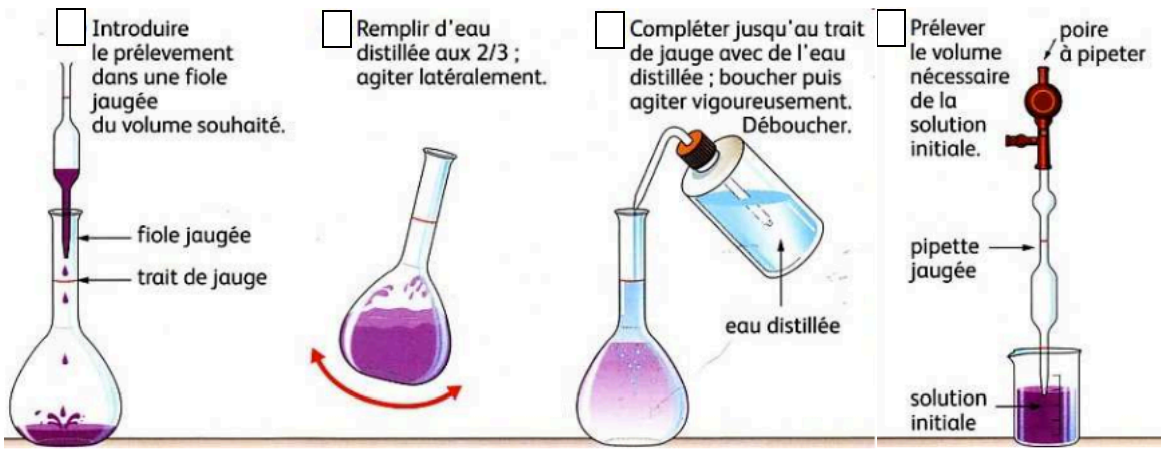
\includegraphics[scale=0.72]{../Chapitre 3 - Puissance consommée par un appareil éléctrique/images/TP6 - dilution.png}
\end{center}
\end{minipage}%
\hfill 
\begin{minipage}{.35\textwidth}%
  \defbox{\fbox{
\begin{minipage}{3cm}{

\textbf{Appel n\degree 1}\\
Appeler M. Ruiz \\ pour vérification  \\[3mm]
Puis réaliser la dilution à l'aide de vos étapes}
\end{minipage}
}}
\end{minipage}%

\vfill

%%%%%%%%%%%%%%%%
\newpage
%%%%%%%%%%%%%%%%

\textbf{\ding{202}  Préparation du dosage} \\

\begin{itemize}
    \item Mettre le bécher étiqueté "récupération de produits usagés" sous la burette.
    \item Vider la burette. 
    \item  Remplir la burette avec la solution de soude (hydroxyde de sodium) de concentration \chemform{C_B = 0,1mol/L }.
    \item Ajuster le niveau du liquide au niveau zéro de la burette en faisant écouler l'excédent de solution
de soude dans le bécher " Récupération de produits usagés".
    
    \item Verser environ 50 mL de la solution de vinaigre diluée dans le bécher étiqueté  Solution A.

    \item Introduire dans le bécher étiqueté "Dosage"
    \begin{itemize}
        \item 10 mL de solution A prélevé à l’aide d’une pipette jaugée propre munie d'un dispositif d’aspiration.
        \item environ 50 mL d'eau distillée
        \item 7 gouttes de BBT
        \item le barreau magnétique propre (le rincer à l'eau distillée puis l'essuyer avec du papier absorbant).
    \end{itemize}
    \item Placer le bécher sous la burette. Agiter doucement la solution à l'aide de l'agitateur magnétique.
    \item Ajouter la solution de soude mL par mL
    \item  Indiquer le volume où apparaît le changement de couleur grâce à un encadrement. On le notera $V_2$.

\begin{minipage}{.6\textwidth}%
    \begin{center}
        \large{.......... mL < $V_2$ < .......... mL}
    \end{center}
\end{minipage}%
\hfill 
\begin{minipage}{.32\textwidth}%
  \defbox{\fbox{
\begin{minipage}{3cm}{
\textbf{Appel n\degree 2}\\Appeler M. Ruiz \\ pour vérification \\ de votre résultat }
\end{minipage}
}}
\end{minipage}%
    


    \item Continuer à verser mL par mL jusqu'à 20 mL.
\end{itemize}

\vfill 

\textbf{\ding{203}  Dosage précis dit goutte à  goutte} \\[3mm]
On recommence le dosage pour déterminer le volume équivalent $V_e$ à la goutte près.
\begin{enumerate}
    \item Recommencer les 3 premières étapes du dosage rapide. 
     \item Introduire dans un erlenmeyer 100 mL, étiqueté "Dosage"
    \begin{itemize}
        \item 10 mL de solution A prélevé à l'aide d’une pipette jaugée propre munie d’un dispositif d’aspiration.
        \item environ 10 mL d'eau distillée
        \item 7 gouttes de BBT
        \item le barreau magnétique propre (le rincer à l'eau distillée puis l'essuyer avec du papier absorbant).
    \end{itemize}
    
    \item Ajouter la solution de soude jusqu'au changement de couleur (point d’équivalence) en
respectant les consignes suivantes : \\
\begin{itemize}
    \item rapidement au début,
     \item puis goutte à goutte à l' approche du changement de couleur (point d’équivalence).
     \item Lire le volume équivalent et inscrire la réponse.
\end{itemize}


\begin{minipage}{.6\textwidth}%
    \begin{center}
        \large  $V_e$ = .......... mL
    \end{center}
\end{minipage}%
\hfill 
\begin{minipage}{.32\textwidth}%
  \defbox{\fbox{
\begin{minipage}{3cm}{\textbf{Appel n\degree 3}\\
Appeler M. Ruiz \\ pour vérification \\ de votre lecture.  }
\end{minipage}
}}
\end{minipage}%

\end{enumerate}

\vfill 


\newpage


\textbf{\ding{204} Rangement du poste de travail}
\begin{itemize}
    \item  Récupérer les contenus des béchers et de la burette dans le bécher marqué " Récupération de
produits usagés ". \textbf{Ne pas jeter à l'évier. }
\item Laver les béchers et erlenmeyers vides avec l'eau du robinet, puis rincer les à l'eau distillée.
\item   Rincer la burette et la pipette à l'eau distillée.
\item  Nettoyer le plan de travail.
\end{itemize}

 \defbox{\fbox{
\begin{minipage}{14cm}{
\textbf{Appel n\degree 4}\\Appeler M. Ruiz pour lui faire vérifier le rangement et lui rendre ce
document. }
\end{minipage}
}}

\textbf{\ding{205} Calcul de \chemform{C_A} }

Calculer la concentration \chemform{C_A} de la solution A (vinaigre) en utilisant la formule : \chemform{C_A \times V_A = C_B \times V_e} 
Rappel : On a dilué 10 fois. 

\vspace{3mm}
\cadreblanc{25}

\vfill 

\textbf{\ding{206} Calcul du degré d'acidité du vinaigre}

Calculer la masse d'acide acétique de formule \chemform{CH_3COOH} présente dans 100 g de vinaigre. 

\cadreblanc{35}

\vfill 

Relever le degré d’acidité porté sur l’étiquette de la bouteille de vinaigre ? Le résultat expérimental
trouvé est-il en accord avec cette valeur ?

\cadreblanc{25}

\vfill 


\end{document}
